%%%%%%%%%%%%%%%%%%%%%%%%%%%%%%%%%%%%%%%%%%%%%%%%%%%%%%%%%%%%%%%%%%%%%%%%%%%%%%%%
\chapter{Компилятор clang и модули для него}
%%%%%%%%%%%%%%%%%%%%%%%%%%%%%%%%%%%%%%%%%%%%%%%%%%%%%%%%%%%%%%%%%%%%%%%%%%%%%%%%

%%%%%%%%%%%%%%%%%%%%%%%%%%%%%%%%%%%%%%%%%%%%%%%%%%%%%%%%%%%%%%%%%%%%%%%%%%%%%%%%
\section{О Clang}
%%%%%%%%%%%%%%%%%%%%%%%%%%%%%%%%%%%%%%%%%%%%%%%%%%%%%%%%%%%%%%%%%%%%%%%%%%%%%%%%
Clang является компилятором для языков программирования C, C++, Objective-C, Objective-C++ и OpenCL.
Для оптимизации исходного кода и затем кодогенерации используется фреймворк LLVM. Хотя Clang разрабатывается
как фронтенд для LLVM, теоретически возможно использовать и другие бэкенды. К примеру в качестве бэкенда
можно использовать GCC. Однако комбинация Clang и LLVM предоставляет набор инструментов, 
позволяющий полностью заменить GCC. 

Разработка Clang началась ввиду того, что был необходим компилятор, который предоставлял бы 
детальные диагностики ошибок, удобную интеграцию с интегрированной средой разработки и имел бы
лицензию, позволяющую использовать компилятор в коммерческих целях. В результате в 2007 году был 
представлен компилятор Clang под лицензий University of Illinois/NCSA Open Source License.
Для интегрированной среды разработки XCode, Clang становится основным компилятором начиная с версии 3.2.
С ноября 2012 года в качестве основного компилятора для FreeBSD используется Clang. Вероятно в ближайшие годы
Clang сменит GCC и будет основным компилятором для языков С и С++ во многих диструбутивах и
других Unix-подобных системах.

Одной из главных целей Clang является поддержка инкрементной компиляции, которая позволяет более
тесно интегрировать компилятор и графический интерфейс среды разработки. Для GCC это непросто 
сделать так как он разрабатывался для использования в классическом цикле "компиляция-линковка-отладка".
Поэтому Clang стремится предоставить фреймворк, позволяющий производить парсинг, индексацию, 
статический анализ и компиляцию языков семейства Си. 

Ввиду того, что изначально Clang был спроектирован для максимального сохранения информации во время 
процесса компиляции, появляется возможность предоставлять контекстно-ориентированные сообщения об ошибках.
Такие сообщения будут понятны программистам и удобны для сред разработки. Так же благодаря 
модульности дизайна компилятора, можно использовать необходимые модули в среде разработки для
индексирования кода, подсветки синтаксиса и рефакторинга.

Подводя итог выше сказанного, можно выделить основные цели использования Clang:

Особенности для конечного пользователя:
\begin{itemize}
\item Быстрая компиляция и небольшое использование памяти
\item Понятные диагностики
\item Совместимость с GCC
\end{itemize}

Преимущества для приложений:
\begin{itemize}
\item Модульная архитектура
\item Поддержка разнообразных инструментов (рефакторинг, статический анализ, генерация кода и так далее)
\item Тесная интеграция с средой разработки
\item Использование BSD-подобной лицензии
\end{itemize}

Внутренний дизайн и реализация:
\begin{itemize}
\item Простой и легко изменяемый исходный код
\item Унифицированный парсер для языков С, Objective-C, C++ и Objective-C++
\item Поддержка последних версий C/C++/Objective-C
\end{itemize}

С полным и подробным списком всех особенностей можно ознакомиться на сайте Clang.

%%%%%%%%%%%%%%%%%%%%%%%%%%%%%%%%%%%%%%%%%%%%%%%%%%%%%%%%%%%%%%%%%%%%%%%%%%%%%%%%
\section{Абстрактное синтаксическое дерево}
%%%%%%%%%%%%%%%%%%%%%%%%%%%%%%%%%%%%%%%%%%%%%%%%%%%%%%%%%%%%%%%%%%%%%%%%%%%%%%%%
Абстрактным синтаксическим деревом (Abstract Syntax Tree) называется представление исходного кода 
в виде дерева, в котором вершинами являются операторы языка программирования, а листья - операндами.
Листья могут представлять только переменные и константы. 

Так как Clang не производит упрощения исходного кода во время компиляции (как это делает GCC),
то гарантируется точное воспроизведение исходного кода в абстрактном синтаксическом дереве, 
что необходимо для полноценного статического анализа. К примеру, скобочные выражения и константы
времени компиляции доступны в исходной форме в абстрактном синтаксическом дереве.

%%%%%%%%%%%%%%%%%%%%%%%%%%%%%%%%%%%%%%%%%%%%%%%%%%%%%%%%%%%%%%%%%%%%%%%%%%%%%%%%
\section{Структура абстрактного синтаксического дерева Clang}
%%%%%%%%%%%%%%%%%%%%%%%%%%%%%%%%%%%%%%%%%%%%%%%%%%%%%%%%%%%%%%%%%%%%%%%%%%%%%%%%
Узлы в абстрактном синтаксическом дереве Clang организованы так, что у них нет общего предка.
Вместо этого, есть несколько больших иерархий классов для простых типов, таких как Decl и Stmt.
\begin{itemize}
	\item Decl представляет объявления (declarations). От данного класса наследуются разнообразные
объявления типов. К примеру класс FunctionDecl отвечает за объявление функции, а класс ParmVarDecl 
за объявление параметра функции.
	\item Stmt представляет операторы (statements). Все классы, описывающие операторы, наследуются
от данного класса. К примеру для оператора "if" существует класс IfStmt, оператору "return" 
соответствует класс ReturnStmt. 
\end{itemize}
Многие важные AST узлы наследуются от классов Type,Decl,DeclContext или Stmt, а некоторые классы 
наследуются от Decl и DeclContext. В Clang AST выражения (expressions) представляются классом Expr,
наследуются от класса Stmt и являются так же операторами. Однако существует множество классов, 
которые не являются частью большой иерархии классов и доступны только из определенных узлов, 
к примеру класс CXXBaseSpecifier. Так же важно помнить, что комментарии не входят в состав 
абстрактного синтаксического дерева.

Все информация о абстрактном синтаксическом дереве для единицы трансляции (translation unit)
собрана в классе ASTContext. Он представляет обход всей единицы трансляции или доступ к таблице
идентификаторов Clang для разобранной единицы трансляции. 

%%%%%%%%%%%%%%%%%%%%%%%%%%%%%%%%%%%%%%%%%%%%%%%%%%%%%%%%%%%%%%%%%%%%%%%%%%%%%%%%
\section{Пример абстрактного синтаксического дерева}
%%%%%%%%%%%%%%%%%%%%%%%%%%%%%%%%%%%%%%%%%%%%%%%%%%%%%%%%%%%%%%%%%%%%%%%%%%%%%%%%
Рассмотрим пример генерации абстрактного синтаксического дерева для следующего кода:
\begin{lstlisting}
int gVar=0;

void func(int arg)
{
	if (arg == 0)
		arg++;

	for (int i=0; i<arg; i++)
		gVar++;
}

int main(int argc, char *argv[])
{
	int arg = 2;
	func(arg);
	return 0;
}
\end{lstlisting}

Для получения абстрактного синтаксического дерева в текстовом виде у Clang есть встроенный 
режим AST-dump, который может быть включен с помощью флага "-ast-dump". Так же отключим кодогенерацию
флагом "-fsyntax-only". В результате для получения AST необходимо ввести в терминал следующую команду:
\begin{lstlisting}
clang -Xclang -ast-dump -fsyntax-only ast.c
\end{lstlisting}
где ast.c - файл с исходным кодом.

В консоль выведется текстовое представление абстрактного синтаксического дерева для приведенного выше исходного кода:
\begin{lstlisting}[basicstyle=\tiny]
TranslationUnitDecl 0x7f8383830ec0 <<invalid sloc>> <invalid sloc>
... внутренние объявления clang ...
|-VarDecl 0x7fc5f98333d0 <ast.c:1:1, col:10> col:5 used gVar 'int' cinit
| `-IntegerLiteral 0x7fc5f9833428 <col:10> 'int' 0
|-FunctionDecl 0x7fc5f9833520 <line:3:1, line:10:1> line:3:6 used func 'void (int)'
| |-ParmVarDecl 0x7fc5f9833460 <col:11, col:15> col:15 used arg 'int'
| `-CompoundStmt 0x7fc5f986fef8 <line:4:1, line:10:1>
|   |-IfStmt 0x7fc5f9833698 <line:5:2, line:6:6>
|   | |-<<<NULL>>>
|   | |-BinaryOperator 0x7fc5f9833628 <line:5:6, col:13> 'int' '=='
|   | | |-ImplicitCastExpr 0x7fc5f9833610 <col:6> 'int' <LValueToRValue>
|   | | | `-DeclRefExpr 0x7fc5f98335c8 <col:6> 'int' lvalue ParmVar 0x7fc5f9833460
'arg' 'int'
|   | | `-IntegerLiteral 0x7fc5f98335f0 <col:13> 'int' 0
|   | |-UnaryOperator 0x7fc5f9833678 <line:6:3, col:6> 'int' postfix '++'
|   | | `-DeclRefExpr 0x7fc5f9833650 <col:3> 'int' lvalue ParmVar 0x7fc5f9833460
'arg' 'int'
|   | `-<<<NULL>>>
|   `-ForStmt 0x7fc5f986feb8 <line:8:2, line:9:7>
|     |-DeclStmt 0x7fc5f9833758 <line:8:7, col:14>
|     | `-VarDecl 0x7fc5f98336e0 <col:7, col:13> col:11 used i 'int' cinit
|     |   `-IntegerLiteral 0x7fc5f9833738 <col:13> 'int' 0
|     |-<<<NULL>>>
|     |-BinaryOperator 0x7fc5f986fe00 <col:16, col:18> 'int' '<'
|     | |-ImplicitCastExpr 0x7fc5f98337c0 <col:16> 'int' <LValueToRValue>
|     | | `-DeclRefExpr 0x7fc5f9833770 <col:16> 'int' lvalue Var 0x7fc5f98336e0
 'i' 'int'
|     | `-ImplicitCastExpr 0x7fc5f98337d8 <col:18> 'int' <LValueToRValue>
|     |   `-DeclRefExpr 0x7fc5f9833798 <col:18> 'int' lvalue ParmVar 0x7fc5f9833460
 'arg' 'int'
|     |-UnaryOperator 0x7fc5f986fe50 <col:23, col:24> 'int' postfix '++'
|     | `-DeclRefExpr 0x7fc5f986fe28 <col:23> 'int' lvalue Var 0x7fc5f98336e0 'i' 'int'
|     `-UnaryOperator 0x7fc5f986fe98 <line:9:3, col:7> 'int' postfix '++'
|       `-DeclRefExpr 0x7fc5f986fe70 <col:3> 'int' lvalue Var 0x7fc5f98333d0
 'gVar' 'int'
`-FunctionDecl 0x7fc5f9870180 <line:12:1, line:17:1> line:12:5 main 'int (int, char **)'
  |-ParmVarDecl 0x7fc5f986ff30 <col:10, col:14> col:14 argc 'int'
  |-ParmVarDecl 0x7fc5f9870070 <col:20, col:31> col:26 argv 'char **':'char **'
  `-CompoundStmt 0x7fc5f98703e8 <line:13:1, line:17:1>
    |-DeclStmt 0x7fc5f98702b8 <line:14:2, col:13>
    | `-VarDecl 0x7fc5f9870240 <col:2, col:12> col:6 used arg 'int' cinit
    |   `-IntegerLiteral 0x7fc5f9870298 <col:12> 'int' 2
    |-CallExpr 0x7fc5f9870360 <line:15:2, col:10> 'void'
    | |-ImplicitCastExpr 0x7fc5f9870348 <col:2> 'void (*)(int)' <FunctionToPointerDecay>
    | | `-DeclRefExpr 0x7fc5f98702d0 <col:2> 'void (int)' Function 0x7fc5f9833520
     'func' 'void (int)'
    | `-ImplicitCastExpr 0x7fc5f9870390 <col:7> 'int' <LValueToRValue>
    |   `-DeclRefExpr 0x7fc5f98702f8 <col:7> 'int' lvalue Var 0x7fc5f9870240
'arg' 'int'
    `-ReturnStmt 0x7fc5f98703c8 <line:16:2, col:9>
      `-IntegerLiteral 0x7fc5f98703a8 <col:9> 'int' 0
\end{lstlisting}

Как видно из текста, корнем абстрактного синтаксического дерева является TranslationUnitDecl.
У данного корня дерева есть несколько вершин:
\begin{itemize}
 \item Внутренние обявления Clang
 \item Объявление глобальной переменной "gVar"
 \item Объявление функции "func"
 \item Объявление функции "main"
\end{itemize}

Рассмотрим подробнее абстрактное синтаксическое дерево для объявления функций "func" и "main". Для этого
на основе приведенного выше текста составим диаграмму вершин Clang AST.
\begin{figure}[H]
\centering
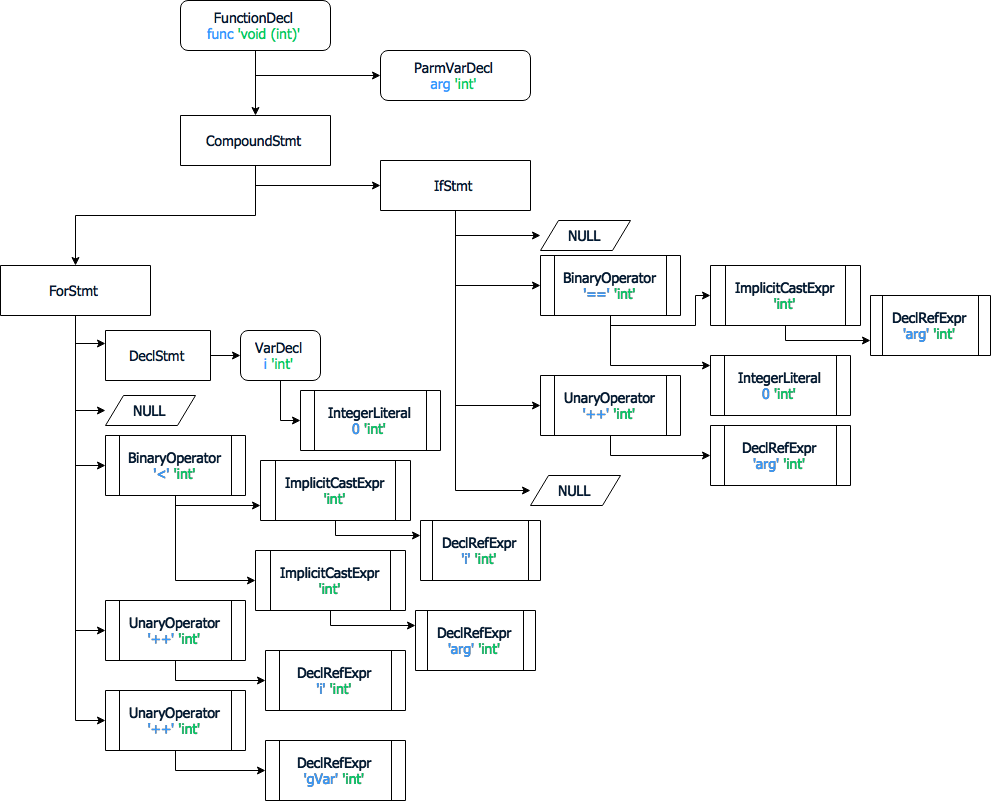
\includegraphics[width=\textwidth]{funcAST}
\caption{Clang AST для объявления функции func}%
\label{fig:funcAST}
\end{figure}
\begin{figure}[H]
\centering
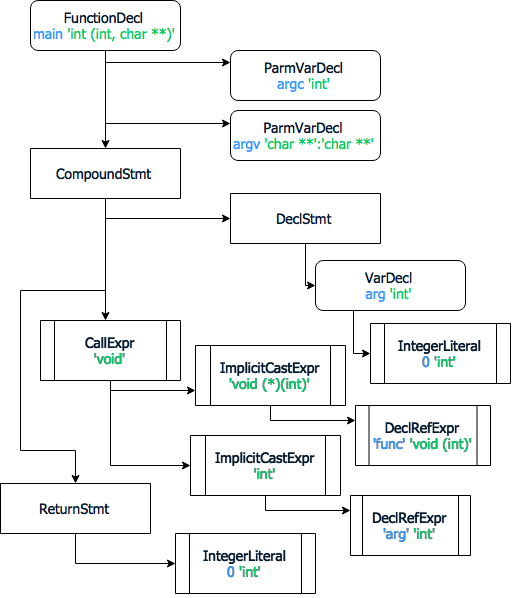
\includegraphics[width=\textwidth]{mainAST}
\caption{Clang AST для объявления функции main}%
\label{fig:mainAST}
\end{figure}

\subsection*{Decl}
Рассмотрим примеры использования типа Decl. Так, для объявления функции, корнем в абстрактном 
синтаксическом дереве должна быть вершина с типом Decl. Из рисунков \ref{fig:funcAST} и \ref{fig:mainAST} 
видно, что корневая вершина имеет тип FunctionDecl, который является подклассом Decl. Данный класс 
отвечает за объявление функции. Если у функции есть параметры, то класс FunctionDecl содержит 
вершины с типом ParmVarDecl, которые отвечают за объявление этих параметров. На рисунке 
\ref{fig:funcAST} функции "func" всего один параметр (arg) и поэтому одна вершина ParmVarDecl, 
в то время как у функции "main" (рисунок \ref{fig:mainAST}) два параметра и 
соответственно две вершины ParmVarDecl. Для объявления локальной или глобальной переменной 
используется VarDecl. На рисунке \ref{fig:funcAST} видно, что для цикла for объявляется переменная "i" типа int,
а на рисунке \ref{fig:mainAST} VarDecl используется для объявления локальной переменной "arg". Так же из
текстового представления абстрактного синтаксического дерева, преведенного выше, видно, что для 
объявления глобальной переменной "gVar" аналогично используется VarDecl. В случае, если у объявляемой 
переменной есть начальное значение, то VarDecl имеет дочернюю вершину с этим значением. В приведенных
примерах дочерней вершиной является вершина с типом IntegerLiteral, которая содержит начальное значение.

\subsection*{Stmt}
Как уже было рассмотрено ранее, Stmt представляет операторы. На рисунках \ref{fig:funcAST} и \ref{fig:mainAST} 
подклассами Stmt являются:
\begin{itemize}
 \item CompoundStmt представляет группу операторов заключенных в фигурные скобки
 \item DeclStmt необходим для определения локальной переменной
 \item ReturnStmt соответсвует оператору "return"
 \item IfStmt соответсвует оператору "if"
 \item ForStmt соответсвует оператору "for"
\end{itemize}

Expr представляет выражения и тоже является подклассом Stmt. На рисунках \ref{fig:funcAST} и \ref{fig:mainAST}
подклассами Expr являются:
\begin{itemize}
 \item CallExpr соответствует вызову функции
 \item ImplicitCastExpr необходим для неявного приведения типов
 \item DeclRefExpr используется для ссылки на объявленные переменные и функции
 \item IntegerLiteral для целых литерал
 \item UnaryOperator и BinaryOperator обозначает унарный и бинарный оператор соответственно 
\end{itemize}
Из абстрактного синтаксического дерева видно, что у оператора может быть несколько дочерних
вершин, которые содержат дополнительную информацию. К примеру у выражения CallExpr может быть несколько вершин:
первая соответствует ссылке на вызываемую функцию, а остальные являются параметрами этой функции.
У BinaryOperator всегда два операнда: левая и правая часть выражения. 
В отличии от операторов (Stmt) у выражений (Expr) есть возвращаемый тип.  

%%%%%%%%%%%%%%%%%%%%%%%%%%%%%%%%%%%%%%%%%%%%%%%%%%%%%%%%%%%%%%%%%%%%%%%%%%%%%%%%
\section{Способы использования Clang}
%%%%%%%%%%%%%%%%%%%%%%%%%%%%%%%%%%%%%%%%%%%%%%%%%%%%%%%%%%%%%%%%%%%%%%%%%%%%%%%%
Clang предоставляет необходимую инфраструктуру для создания инструментов, которым необходима
синтаксическая и семантическая информация из исходного кода. Для того, чтобы использовать все 
возможности Clang есть три способа создания инструментов: использование библиотеки LibClang, 
использование библиотеки LibTooling или создание плагина для Clang. Рассмотрим каждый из методов.

\subsection*{LibClang}
LibClang представляет стабильный высокоуровневый интерфейс к Clang, написанный на языке С. 
Является хорошим выбором если необходим стабильный API, так как Clang периодически меняется.
В случае если использовать LibTooling или создавать плагин, то нужно обновлять написанный код,
чтобы он соответствовал изменениям в Clang. Так же LibClang позволяет использовать другие языки
программирования для доступа к Clang API, а не только С++. Однако LibClang не предоставляет полного доступа к 
абстрактному синтаксическому дереву, только высокоуровневый доступ.

\subsection*{LibTooling}
LibTooling это С++ интерфейс, используемый для написания отдельного приложения. Типовые примеры использования
LibTooling:
\begin{itemize}
	\item Простой контролер синтаксиса
	\item Инструменты рефакторинга
\end{itemize}
 
В отличии от LibClang, предоставляется полный доступ к абстрактному синтаксическому дереву. 
Анализировать можно как один файл, так и заданный набор файлов, независимо от системы сборки.

Примерами использования LibTooling являются Clang Tools. Clang Tools - это коллекция специальных 
инструментов для разработчика, используемых для автоматизации и улучшения разработки на языках C и C++.
Примеры созданных или планируемых инструментов как часть проекта Clang:
\begin{itemize}
	\item Проекра синтаксиса (clang-check)
	\item Автоматическое исправление ошибок компиляции (clang-fixit)
	\item Автоматическое форматирование кода (clang-format)
	\item Инструменты для миграции кода под новый стандарт языка (clang-modernize)
	\item Инструменты для рефакторинга
\end{itemize}

\subsection*{Плагин для Clang}
Использование плагина для Clang позволяет производить дополнительные действия при обходе абстрактного 
синтаксического дерева как часть процесса компиляции. Плагины представляют из себя динамические
библиотеки, которые могут подключаться к компилятору во время выполнения. Благодоря динамическому подключению 
к компилятору, плагин легко интегрировать в среду сборки проекта. Так же плагин имеет возможность 
останавливать процесс сборки. Как и при использовании LibTooling, плагину предоставляется полный
контроль над абстрактным синтаксическим деревом.
 
Однако стоит помнить, что нецелесообразно создавать плагин, если:
\begin{itemize}
	\item Необходимо использовать плагин вне среды сборки
	\item Необходимо использовать плагин для определенного набора файлов в проекте, которые 
не обязательно вызывают пересборку проекта
\end{itemize}

%%%%%%%%%%%%%%%%%%%%%%%%%%%%%%%%%%%%%%%%%%%%%%%%%%%%%%%%%%%%%%%%%%%%%%%%%%%%%%%%
\section{RecursiveASTVisitor и ASTMatcher}
%%%%%%%%%%%%%%%%%%%%%%%%%%%%%%%%%%%%%%%%%%%%%%%%%%%%%%%%%%%%%%%%%%%%%%%%%%%%%%%%
Для обхода и нахождения интересующих мест в абстрактном синтаксическом дереве Clang есть два подхода:
используя RecursiveASTVisitor и с помощью AST Matchers.

Рассмотрим как с помощью каждого подхода найти интересующий фрагмент кода. В качестве примера
будет рассмотрено нахождение фрагмента кода, содержащий оператор if и в качестве условия 
происходит сравнение указателя и 0:
\begin{lstlisting}
int main()
{
	int var = 5;
	int *ptr = &var;
	if (ptr < 0) // <==
		var++;
	return 0;
}
\end{lstlisting}

Абстрактное синтаксическое дерево для интересующего фрагмента кода:
\begin{lstlisting}[basicstyle=\tiny]
-IfStmt 0x7fdb75024790 <line:18:2, line:19:6>
|-<<<NULL>>>
|-BinaryOperator 0x7fdb75024720 <line:18:6, col:12> 'int' '<'
| |-ImplicitCastExpr 0x7fdb750246f0 <col:6> 'int *' <LValueToRValue>
| | `-DeclRefExpr 0x7fdb750246a8 <col:6> 'int *' lvalue Var 0x7fdb750245f0 'ptr' 'int *'
| `-ImplicitCastExpr 0x7fdb75024708 <col:12> 'int *' <NullToPointer>
|   `-IntegerLiteral 0x7fdb750246d0 <col:12> 'int' 0
|-UnaryOperator 0x7fdb75024770 <line:19:3, col:6> 'int *' postfix '++'
| `-DeclRefExpr 0x7fdb75024748 <col:3> 'int *' lvalue Var 0x7fdb750245f0 'ptr' 'int *'
`-<<<NULL>>>
\end{lstlisting}

\subsection*{RecursiveASTVisitor}
Класс RecursiveASTVisitor позволяет обойти каждую вершину абстрактного синтаксического дерева.
Для этого необходимо создать класс, который будет отвечать за обход абстрактного синтаксического 
дерева. Данный класс должен наследоваться от класса RecursiveASTVisitor. Чтобы обойти интересующие вершины,
достаточно переопределить функцию "bool VisitNodeType(NodeType *)". Так для обхода всех Stmt 
необходимо переопределить функцию "bool VisitStmt(Stmt *)". Так же можно переопределить функцию
для поиска вершин, которые являются подклассами Stmt. К примеру для нахождения оператора "if"
нужно переопределить функцию "bool VisitIfStmt(IfStmt *)". В этом случае для оператора "if" 
будет вызываться два обработчика: VisitStmt и VisitIfStmt.

Для Visit* функций необходимо возвращать значение "true", чтобы продолжить обход остальных вершин
абстрактного синтаксического дерева. Если же возвратить значение "false", обход дерева полностью
прекращается и Clang завершает работу.

Рассмотрим как стоит использовать RecursiveASTVisitor для нахождения участка кода из вышеописанного
примера.

Проанализировав полученное для исходного кода абстрактное синтаксическое дерево видно, что 
корнем для искомого фрагмента является IfStmt. Поэтому в классе, созданном для обхода AST
следует переопределить функцию с именем "VisitIfStmt". Так же нетрудно заметить, что условием 
оператора "if" должен быть оператор сравнения (BinaryOperator), в котором в левой части
находится указатель, а в правой константа, равная 0. Между левой и правой частью оператора сравнения
должен быть символ "<". Основываясь на вышесказанном, можно написать код, для выявления заданного шаблона.
\begin{lstlisting}
class Example:
	public RecursiveASTVisitor<Example> 
{
public:
bool VisitIfStmt(IfStmt *s) {
  if (const BinaryOperator *binOP =
          llvm::dyn_cast<BinaryOperator>(s->getCond())) 
  {
    if (binOP->getOpcode() == BO_LT) 
    {
      const Expr *LHS = binOP->getLHS();
      if (const ImplicitCastExpr *Cast =
              llvm::dyn_cast<ImplicitCastExpr>(LHS)) 
      {
        LHS = Cast->getSubExpr();
      }
      
      const Expr *RHS = binOP->getRHS();
      if (const ImplicitCastExpr *Cast =
              llvm::dyn_cast<ImplicitCastExpr>(RHS)) 
      {
        RHS = Cast->getSubExpr();
      } 

      if (
const DeclRefExpr *dRef=llvm::dyn_cast<DeclRefExpr>(LHS) &&
const IntegerLiteral *intVal = 
		llvm::dyn_cast<IntegerLiteral>(RHS)) 
	  {
        if (const VarDecl *Var =
                llvm::dyn_cast<VarDecl>(dRef->getDecl())) 
        {
          if (Var->getType()->isPointerType() &&
              intVal->getValue().getZExtValue() == 0) 
          {
            s->dump();  // found
          }
        }
      }
    }
  }
  return true;
}
};
\end{lstlisting}

Как видно для нахождения простого шаблона нужно написать довольно много кода. Главной проблемой 
является то, что данный код трудно читать. Чтобы понять, какой шаблон ищет приведенный код,
необходимо вчитываться и смотреть, что делает каждая строчка кода. Намного лучше для выявления 
шаблонов использовать ASTMatcher.


\subsection*{ASTMatcher}
С недавного временив Clang появилась библиотека ASTMatcher, которая предоставляет простой, мощный и
краткий способ определенные шаблоны в абстрактном синтаксическом дереве. Реализованные как
предметно ориентированный язык на основе макросов и шаблонов, matchers похожи на алгебраические 
типы данных из функциональных языков программирования.

К примеру для исследования только бинарных операторов есть matcher который делает именно это и называется 
"binaryOperator". Для того, чтобы исследовать только бинарный оператор, в левой части у которого 
используется литера 0, необходимо написать следующий matcher: 
\begin{lstlisting}
binaryOperator(hasLHS(integerLiteral(equals(0))))
\end{lstlisting}
Данный matcher не будет находить фрагменты кода, где используются другие формы 0, такие как '\textbackslash0' или NULL,
но matcher будет работать, если используется макрос, который раскрывается в 0. Matcher так же 
не будет срабатывать если используется перегруженный бинарный оператор, так как для этого 
есть специальный matcher, который называется "operatorCallExpr" и используется для обработки 
перегруженных операторов. 

Есть три простых категории для matchers:
\begin{enumerate}
	\item \textit{Node Matchers.} Используются для поиска в AST по определенному типу. Любой шаблон
определяющий выражение должен начинаться с Node Matcher, который затем можно уточнить с помощью
Narrowing Matcher или Traversal Matcher. Все Traversal Matcher используют Node Matcher в качестве аргументов.
Так же только Node Matcher имеют метод "bind" для связывания заданного узла и имени, для того чтобы в дальнейшем
можно было получить найденный узел по имени.
	\item \textit{Narrowing Matchers.} Используются для поиска по атрибутам вершины абстрактного
синтаксического дерева. Есть специальные логические Narrowing Matchers которые позволяют 
пользователям более мощные выражения. 
	\item \textit{Traversal Matchers.} Используются для нахождения узла по связям между узлами 
абстрактного синтаксического дерева. Есть специальные Traversal Matchers которые работают для 
всех узлов и позволяют пользователям писать более универсальные выражения.
\end{enumerate}
Для полного списка всех доступных AST Matchers смотрите документацию.

Если Matcher описывает сущность в абстрактном синтаксическом дереве Clang и может быть 
связан с именем, то на него можно получить ссылку когда шаблон найден. Для этого нужно
вызвать метод "bind" на нужном шаблоне. К примеру следующий шаблон находит все переменные типа
int и связывает с этой переменной имя "intVar":
\begin{lstlisting}
variable(hasType(isInteger())).bind("intvar")
\end{lstlisting}

Для обработки фрагментов кода, удовлетворяющих заданному шаблону необходимо создать класс обработчик.
Данный класс должен наследоваться от класса MatchCallback. Класс MatchCallback является вложенным
классом для класса MatchFinder. У класса MatchCallback есть три функции, которые можно переопределить:
\begin{enumerate}
	\item \textbf{void run(const MatchResult \&Result)}. Является обязательной для переопределения.
Вызов данной функции происходит каждый раз, когда был найден участок кода, соответствующий
заданному шаблону
	\item \textbf{void onStartOfTranslationUnit()}. В отличии от функции "void run(const MatchResult \&Result)"
данная функция не является обязательной для переопределения. Вызывается каждый раз в начале
разбора для каждой единицы трансляции
	\item \textbf{void onEndOfTranslationUnit()}. Функция "void onEndOfTranslationUnit()"
аналогична ранее рассмотренной функции "void onStartOfTranslationUnit()" с единственным отличием,
что вызывается каждый раз в конце разбора для каждой единицы трансляции.
\end{enumerate}

Как видно из заголовка функции "run", в качестве параметра данной функции передается ссылка
на результат класс MatchResult. Данный класс необходим для получения всей информации при
совпадении абстрактного синтаксического дерева с заданным шаблоном. 

За работу по нахождению участков кода, соответствующих заданному шаблону отвечает класс
MatchFinder. Для регистрации обработчика и шаблона, который данный обработчик будет анализировать
необходимо использовать функцию \textit{addMatcher}. Первым параметром данной функции является 
шаблон который необходимо выявить в абстрактном синтаксическом дереве. Вторым параметром необходимо
передать указатель на экземпляр класса обработчика. 

Рассмотрим насколько просто нахождение участка кода из вышеописанного примера нахождения сравнения указателя
и 0 с использованием ASTMatcher.

Как уже было рассмотрено ранее, корнем для искомого фрагмента кода должен быть IfStmt обозначающий
оператор "if". Затем условием оператора "if" должен быть оператор сравнения (BinaryOperator), 
в левой части которого находится указатель, а в правой литера 0. В результате AST matcher будет
выглядеть следующим образом: 
\begin{lstlisting}
ifStmt( hasCondition( binaryOperator(
	hasOperatorName("<"),
	hasLHS(ignoringParenImpCasts(declRefExpr(
    to(varDecl(hasType(pointsTo(AnyType))).bind("lhs"))))),
    hasRHS(ignoringParenImpCasts(integerLiteral(equals(0))))
    ))).bind("if")
\end{lstlisting}

Обработчик, вызываемый при нахождении данного совпадения выглядит так:
\begin{lstlisting}
class Example:
public MatchFinder::MatchCallback 
{
public:
virtual void run(const MatchFinder::MatchResult &Result) 
{
const IfStmt *s = Result.Nodes.getNodeAs<clang::IfStmt>("if");
    if (s)
      s->dump();
  }
};
\end{lstlisting}

Как видно необходимо писать намного меньше кода, чем при использовании RecursiveASTVisitor,
вследствии чего труднее допустить ошибки. Так же важным преимуществом использования AST Matcher
является наглядность. Увидев такой шаблон, можно сразу понять какому исходному коду он соответствует. 
